\documentclass[conference]{IEEEtran}
\IEEEoverridecommandlockouts

% Essential Packages
\usepackage{amsmath}
\usepackage{amsthm}
\usepackage{amsfonts}
\usepackage{amssymb}
\usepackage{graphicx}
\usepackage{caption}
\usepackage{subcaption}
\usepackage{algorithm}
\usepackage{algorithmic}
\usepackage{float}
\usepackage{booktabs}
\usepackage[colorlinks, citecolor=blue]{hyperref}
\usepackage{balance}
\usepackage{xcolor}
\usepackage{cleveref}
\usepackage{placeins}

\usepackage[normalem]{ulem}
\newcommand{\rev}[1]{\textcolor{blue}{#1}}

% Compact float spacing for the 8-page limit
\setlength{\textfloatsep}{9pt plus 2pt minus 3pt}
\setlength{\dbltextfloatsep}{9pt plus 2pt minus 3pt}
\setlength{\floatsep}{8pt plus 2pt minus 2pt}
\setlength{\intextsep}{8pt plus 2pt minus 2pt}
\setlength{\abovecaptionskip}{4pt}
\setlength{\belowcaptionskip}{0pt}

% Theorem-like environments
\newtheorem{lemma}{Lemma}
\newtheorem{theorem}{Theorem}
\newtheorem{observation}{Observation}
\newtheorem{definition}{Definition}

\title{Data-Aware Task Scheduling for Approximate DAG Workflows in Federated Fog Systems}
\author{
\IEEEauthorblockN{Gayani Gupta\IEEEauthorrefmark{1}, Amisha Gupta\IEEEauthorrefmark{2},
Mohsen Amini Salehi\IEEEauthorrefmark{1},\\
Antonio Fern\'andez Anta\IEEEauthorrefmark{3},\IEEEauthorrefmark{4},
Sanjukta Bhowmick\IEEEauthorrefmark{1}, Jos\'e Aguilar\IEEEauthorrefmark{4},\IEEEauthorrefmark{5}}
\IEEEauthorblockA{\IEEEauthorrefmark{1}University of North Texas, USA\quad
\IEEEauthorrefmark{2}UC Berkeley, USA\quad
\IEEEauthorrefmark{3}IMDEA Networks Institute, Spain\\
\IEEEauthorrefmark{4}IMDEA Software Institute, Spain\quad
\IEEEauthorrefmark{5}Universidad de Los Andes, Venezuela\quad
gayani.gupta@unt.edu}
}

\date{}

\begin{document}

\maketitle

\begin{abstract}
Flood forecasting, wildfire tracking, and evacuation planning all run as workflows of dependent tasks. During an extreme event, the cloud link often fails, so the work must be done on small fog computers near the disaster area. A single fog site rarely has enough capacity to finish in time, but nearby sites can still reach each other through fast links, so a federation of them is the natural place to run the workflow. Scheduling on a federation is difficult for two reasons. First, a task's input data can take as long to arrive as the task takes to run. Second, many tasks can be run approximately: they give a less accurate result in less time, which is often the right trade-off under a deadline.

We write this scheduling problem as a mixed-integer linear program (MILP) that decides which fog node runs each task and how much of it runs, maximizing the workflow's average accuracy subject to its deadline. The model takes per-edge data sizes and per-link bandwidths as inputs; to our knowledge, no earlier model treats these inputs and these two decisions together. Since the MILP is only practical at moderate sizes, we also build three faster schedulers on the same cost model---linear-program (LP) relaxation with randomized rounding, a bandwidth-aware greedy rule, and a genetic algorithm---and compare all four in simulation. Under tight deadlines the MILP wins by a clear margin; with generous slack the MILP and the greedy both reach the accuracy bound; and at the largest sizes the simple greedy is nearly as good while running far faster.
\end{abstract}

\begin{IEEEkeywords}
Data-aware scheduling, federated fog systems, directed acyclic graphs, approximate computing, mixed-integer linear programming, genetic algorithms.
\end{IEEEkeywords}

\section{Introduction}

Industrial and emergency applications increasingly run on fog computers: small compute sites close to the sensors, deployed where the data is produced. This is especially important in remote or extreme environments like offshore platforms, deep-sea facilities, or disaster zones, where the link to a cloud data center is slow, intermittent, or simply absent. When the cloud cannot be reached, a local fog site must handle time-critical work on its own, and a single site often does not have enough capacity to finish a workflow before its deadline.

A practical way to add capacity is to federate nearby fog sites. During a wildfire, for example, the computers at an evacuation shelter, a field hospital, and a mobile command unit can still reach each other over local radio links even when the wide-area network is down. A federated fog then works like a small local cloud: tasks can be placed on any node, and nodes share data over the inter-fog links \cite{fgcs2024,hong2019survey}.

Federation, however, makes scheduling harder, not easier. Real-time industrial applications are usually written as directed acyclic graphs (DAGs), where an edge means that one task must receive another task's output before it can start. Those edges carry real data, such as sensor streams, simulation checkpoints, or model features. Moving that data between nodes takes time that depends on the link bandwidth. Most existing fog schedulers reason only about compute: they ask where a task runs fastest, but not how long it takes to get the task's input there. In a disaster-response workflow, this omission is costly because a ``fast'' remote placement can lose more time to data transfer than it saves in execution.

There is a second factor that data-unaware schedulers also ignore: tasks can run approximately. Many analytics tasks produce a less accurate result in less time: sampling a simulation fewer times, truncating a feature pipeline, or stopping an iterative method early. When a deadline is tight, running a task at 80\% accuracy may be the difference between a warning that arrives in time and one that arrives too late.

This paper integrates both aspects into one scheduling model. The contributions are:

\begin{itemize}
    \item A data- and bandwidth-aware formulation of approximate DAG scheduling in federated fog systems as a mixed-integer linear program (MILP, Section~\ref{sec:model}): maximize average accuracy under precedence, communication delay, placement eligibility, and one workflow deadline. To our knowledge, per-edge data size, per-link bandwidth, and per-task execution fraction have not previously been modeled jointly in this setting.
    \item Three scalable schedulers on the same cost model: LP relaxation with randomized rounding, a bandwidth/data-aware greedy algorithm, and a genetic algorithm (Section~\ref{sec:algorithms}).
    \item A simulation study varying deadline slack, fog-network size, workflow size, task failure rate, and link bandwidth (Section~\ref{sec:evaluation}).
    \item A correctness argument and a linearization suitable for standard MILP solvers (the Appendix).
\end{itemize}

An earlier version of the scheduling model appeared in a conference paper~\cite{gupta2025efficient}; this work adds the complete data- and bandwidth-aware formulation with proofs and linearization, the failure-rate and bandwidth-degradation experiments, and the comparison against a bandwidth-blind baseline.

%\red{Concretely, relative to~\cite{gupta2025efficient} this paper contributes (i) the complete joint formulation in which per-edge data sizes and per-link bandwidths enter as inputs and per-task execution fractions are decision terms; (ii) the correctness argument and big-$M$ linearization of Appendix~\ref{app:proofs}; (iii) the failure-rate and bandwidth-degradation experiments; and (iv) the comparison against a bandwidth-blind baseline that isolates the value of the data-aware terms.}

\section{Related Work}
\label{sec:related}

Scheduling a DAG of tasks on heterogeneous processors is a well-studied
problem. The standard reference heuristic is HEFT \cite{topcuoglu2002heft},
which ranks each task by the remaining work plus communication on the
longest path to the end of the graph and places each task, in rank order,
on the processor where it finishes earliest. Our model uses the same
convention that the transfer cost lives on the DAG edge. The difference
is what a task is allowed to be: HEFT assumes a task runs completely or
not at all, and so do the DAG schedulers used in mobile edge computing
\cite{li2023dagmec} and the learned schedulers built on graph neural
networks \cite{sharma2025grapheonrl}. In our model a task can run
partially; the execution fraction $l_{ia}$ is a decision variable, so a
workflow that cannot finish at full quality can still finish with less
accuracy. Partitioning a task graph for data-intensive workflows has
been studied before \cite{ahmad2014workflow}, but without per-link
bandwidth or partial execution.

Fog and edge resource allocation is surveyed in \cite{hong2019survey,mao2017survey}, and federating nearby fog sites has been proposed for industrial settings \cite{fgcs2024}. Inside such a federation, existing schedulers mostly worry about compute: where to place components for throughput \cite{faticanti2020partitioning} or how to meet quality-of-service targets \cite{russo2024qos}. What they largely ignore is the data that must travel between dependent tasks. In a federated fog the links between sites are the scarce resource, so a scheduler that ignores them can pick a plan that looks fast on paper but misses its deadline in the field. Our formulation avoids that by putting the data volume on every edge and the bandwidth on every link directly into the optimization, together with partial execution.

Trading result quality for resources is not new. Probabilistic task
pruning drops low-value tasks to keep a schedule feasible under load
\cite{gentry2019taskpruning}, and stochastic optimization makes
allocations robust to uncertain runtimes \cite{Salehi2016}. We use a
softer version: instead of dropping a task, the scheduler can run part
of it. That difference matters in disaster response, where dropping the
alerting task is not an option but running a faster, slightly less
accurate version of it may be.

\section{System Model and Problem Statement}
\label{sec:model}

\subsection{Setting}

We consider a federation of fog nodes $F=\{f_1,\ldots,f_m\}$ deployed across a wildfire-prone region---a gateway at the field station, a shelter, a hospital, and a mobile response unit (Fig.~\ref{fig:architecture}). Each pair of nodes is connected by a link of known bandwidth, and the federation keeps working when the link to the cloud is down, which during a fire is the common case rather than the exception. A workflow arrives as a DAG $G=(T,E)$, where each node $T_i\in T$ is a computational task, and each edge $(T_j,T_i)\in E$ is both a precedence constraint and a data transfer of size $D_{ji}$.

\begin{figure*}[t]
\centering
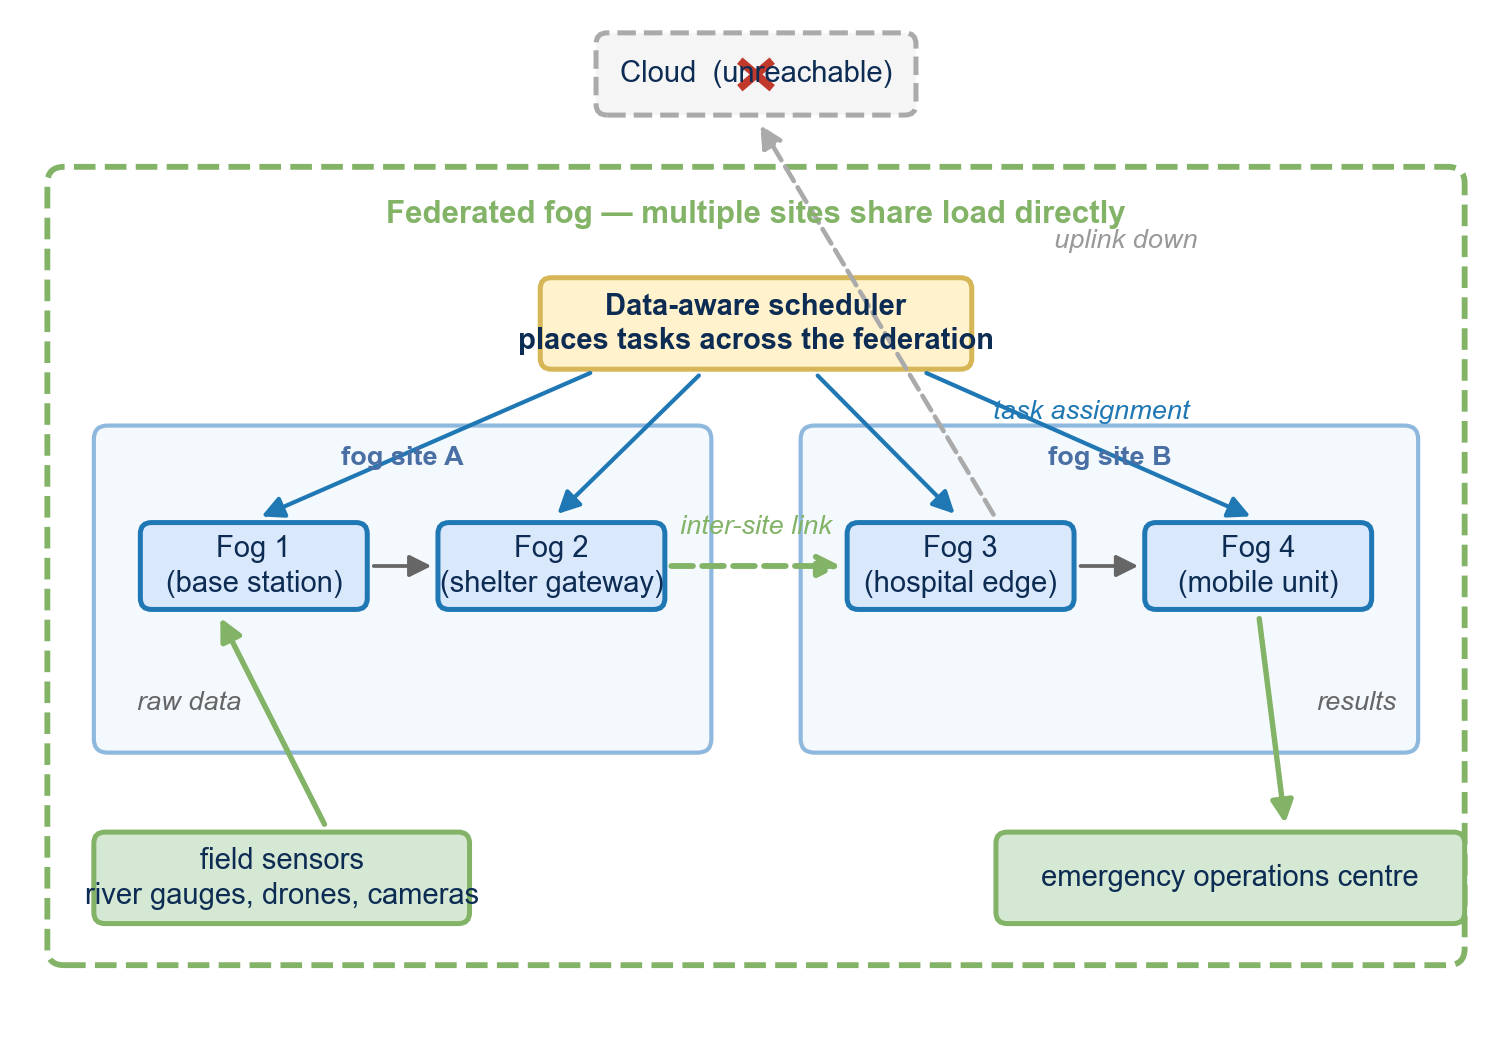
\includegraphics[width=0.72\textwidth]{Figures/federated-fog-architecture.png}
\caption{Federated fog deployment for wildfire response. Smoke cameras, drones, and weather stations feed a workflow of dependent tasks; the scheduler assigns each task to one fog node ($f_1$ Gateway, $f_2$ Shelter, $f_3$ Hospital, $f_4$ Mobile --- the same nodes as Fig.~\ref{fig:dag}), priced by both compute time and inter-node data-transfer cost.}
\label{fig:architecture}
\end{figure*}

If task $T_j$ runs on node $f_b$ and its successor $T_i$ runs on node $f_a$, the input of $T_i$ has to cross the link $(f_b,f_a)$ with bandwidth $B_{ba}$. That transfer takes:
\begin{equation}
 c_{ji}^{ba}=\begin{cases}
 0, & f_b=f_a,\\[2pt]
 \dfrac{D_{ji}}{B_{ba}}, & f_b\neq f_a.
 \end{cases}
\label{eq:comm}
\end{equation}
This is the central cost in the model: placing a task is not only about how fast a node computes, but also about how long its input data take to arrive.

\begin{figure}[h!]
\centering
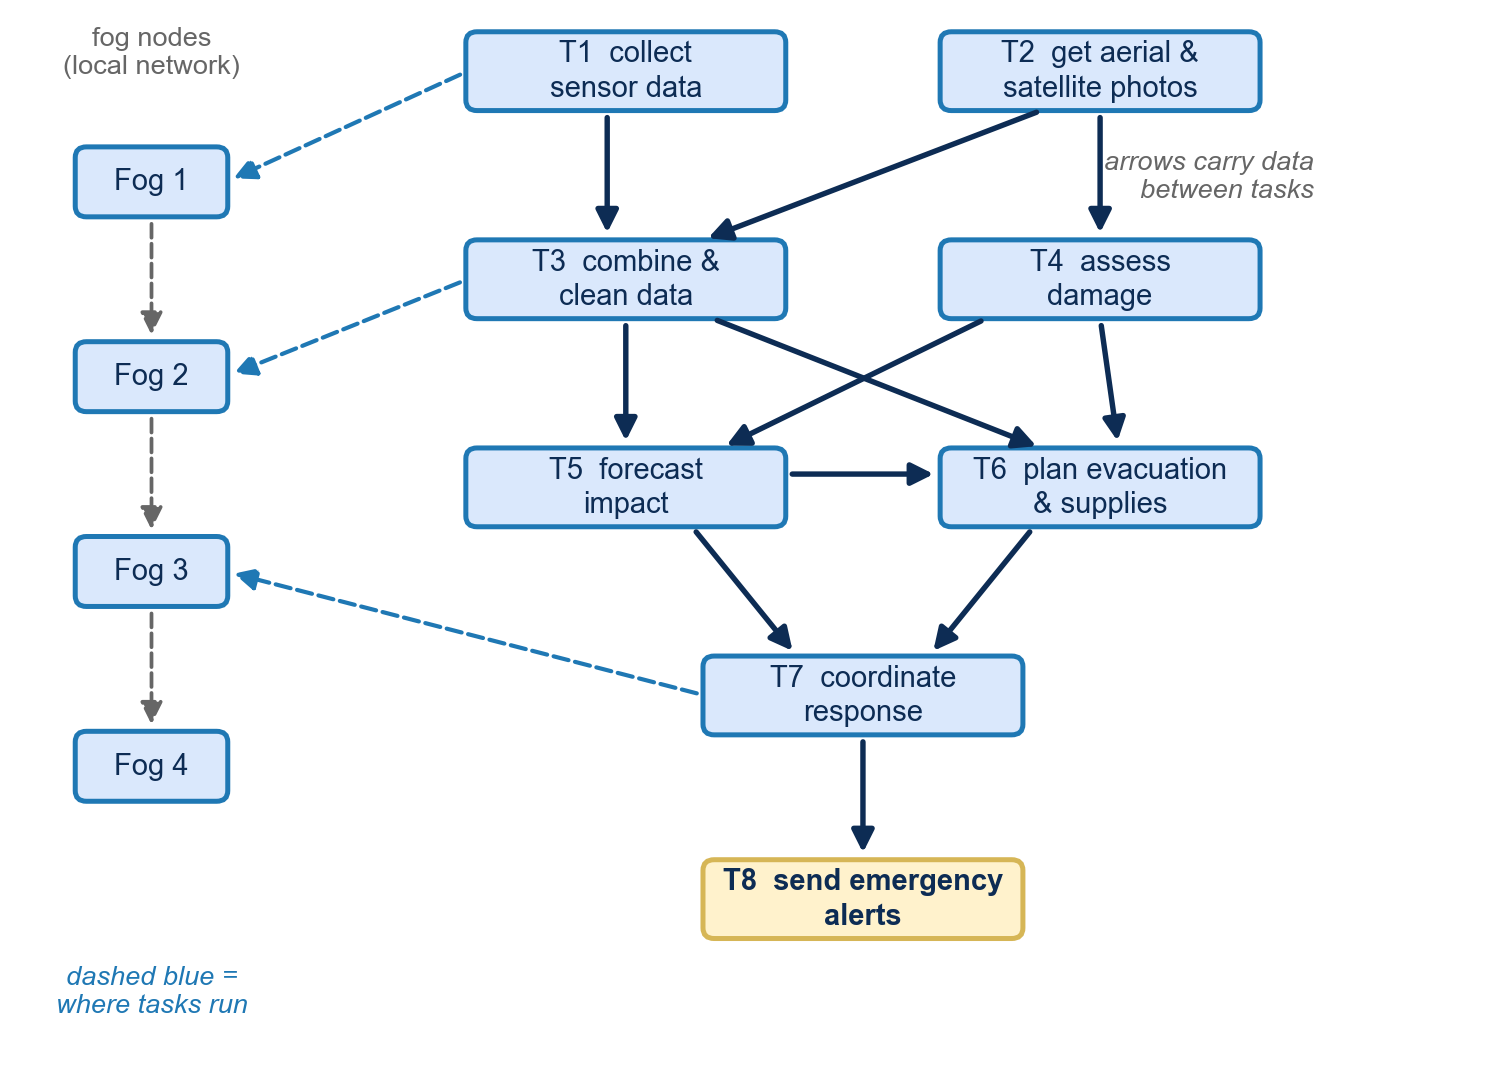
\includegraphics[width=\linewidth]{Figures/disaster-response-dag.png}
\caption{A wildfire-response workflow (a) mapped onto a federated fog network (b): imagery is ingested, environmental data prepared, smoke detected, the fire spread predicted and mapped, and damage assessed. Edge labels are data sizes $D_{ji}$; link labels are bandwidths $B_{ba}$; the fog node inside each task shows its placement $e_{ia}$. The highlighted transfer---smoke-detection frames $T_3$ on $f_1$ feeding spread prediction $T_4$ on $f_3$---pays $D_{ji}/B_{ba} = 14400\,\mathrm{Mb}/80\,\mathrm{Mbp/s} = 180\,\mathrm{s}$ (1800 MB expressed in megabits), the transfer delay of Eq.~\eqref{eq:comm}.}
\label{fig:dag}
\end{figure}

\subsection{Assumptions}
Tasks are non-preemptive, each task runs on at most one node, inputs from
all predecessors can arrive in parallel when the links allow it, and
concurrent tasks on the same node do not slow each other down. The
important assumption is the last one: a task can run approximately, and
executing fraction $l$ of it costs fraction $l$ of its full time and
earns fraction $l$ of its accuracy. \rev{Running $T_i$ at $l_{ia}{=}0.5$
produces half of a full-quality result---an iterative solver stopped
after half its iterations, a video pipeline processing every other
frame. This linear trade-off is a first-order model, not a law, but it
makes the deadline--accuracy trade-off explicit and keeps
\eqref{eq:obj}--\eqref{eq:bin} linear.}

\subsection{The Scheduling Problem}

Table~\ref{tab:notation} lists the notation. Each task $T_i$ has a full-accuracy value $A_i$, an execution time $t_{ia}$ on each node $f_a$, and a placement-eligibility indicator $P_{ia}$. The workflow must finish by a deadline $t_{\max}$.

\begin{table}[t]
\centering
\caption{Parameters and decision variables.}
\label{tab:notation}
\small
\begin{tabular}{ll}
\toprule
\textbf{Symbol} & \textbf{Meaning} \\
\midrule
$T_i$ & task $i$ of the workflow DAG \\
$f_a$ & fog node $a$ \\
$t_{ia}$ & full execution time of $T_i$ on $f_a$ \\
$A_i$ & accuracy delivered if $T_i$ runs completely \\
$D_{ji}$ & data transferred from $T_j$ to $T_i$ \\
$B_{ba}$ & bandwidth of link $(f_b,f_a)$ \\
$P_{ia}$ & $1$ if $T_i$ may run on $f_a$, else $0$ \\
$\mathrm{in}_i$ & predecessors of $T_i$ in the DAG \\
$t_{\max}$ & workflow deadline \\
\midrule
$e_{ia}$ & $1$ if $T_i$ is assigned to $f_a$ \\
$l_{ia}$ & fraction of $T_i$ executed on $f_a$ \\
$M_{ia}$ & earliest time $T_i$ can start on $f_a$ \\
$y_i$ & completion time of $T_i$ \\
\bottomrule
\end{tabular}
\end{table}

The problem is then to choose, for every task, which node runs it and how much of it runs, so that the average delivered accuracy is as high as possible and that every task finishes by $t_{\max}$.

\subsection{MILP Formulation}
\label{sec:milp}

The objective is to maximize the average accuracy over the workflow:
\begin{equation}
 \max \quad \frac{1}{n}\sum_{T_i\in T}\; A_i\sum_{f_a\in F} l_{ia}.
\label{eq:obj}
\end{equation}
subject to
\begin{align}
 &\sum_{f_a\in F} e_{ia} =1, && \forall T_i\in T, \label{eq:one}\\
 &e_{ia} \le P_{ia}, && \forall T_i,\ f_a, \label{eq:elig}\\
 &0 \le l_{ia} \le e_{ia}, && \forall T_i,\ f_a, \label{eq:frac}\\
 &M_{ia} \ge y_j+\sum_{f_b\in F} e_{jb}\,c_{ji}^{ba}, && \forall f_a,\ \forall T_i,\ \forall T_j\in\mathrm{in}_i, \label{eq:start}\\
 &M_{ia} =0, && \forall f_a,\ T_i:\mathrm{in}_i=\varnothing, \label{eq:startsrc}\\
 &y_i =\sum_{f_a\in F} e_{ia}\bigl(M_{ia}+t_{ia}l_{ia}\bigr), && \forall T_i, \label{eq:compl}\\
 &y_i \le t_{\max}, && \forall T_i, \label{eq:deadline}\\
 &e_{ia} \in\{0,1\}. && \label{eq:bin}
\end{align}

Constraints \eqref{eq:one}--\eqref{eq:elig} place every task on exactly one permitted node. Constraint \eqref{eq:frac} ties the execution fraction to the assignment: a task can only run where it is placed, and at most one $l_{ia}$ per task is non-zero. \rev{The case $l_{ia}=0$ means the task is placed but never runs; it earns no accuracy, but it still hands its output data $D_{ji}$ to every successor, so the transfer cost in \eqref{eq:comm} is charged whether or not the task ran. Skipping is rare in practice (Fig.~\ref{fig:skipped}); every certified-optimal run executes all tasks at least partially.} Constraint \eqref{eq:start} is the data-aware term: a task cannot start before every predecessor has finished \emph{and} its output has crossed the link. Equation \eqref{eq:compl} defines the completion time and \eqref{eq:deadline} enforces the deadline. The products $e_{ia}M_{ia}$ in \eqref{eq:compl} are quadratic; the Appendix gives the standard linearization ($z_{ia}=e_{ia}M_{ia}$) and the correctness argument.

Scheduling problems of this kind are NP-hard already on unrelated
parallel machines \cite{lenstra1990approximation}, so we treat the MILP
as the benchmark: it gives the best achievable accuracy on instances
small enough to solve exactly and defines the constraints every scalable
method must respect. For larger workflows we use three cheaper methods:
randomized rounding \cite{raghavan1987randomized}, a greedy scheduler,
and a genetic algorithm.

\section{Scalable Scheduling Algorithms}
\label{sec:algorithms}

All three methods take the same inputs as the MILP: the DAG, the times $t_{ia}$, the data sizes $D_{ji}$, the bandwidths $B_{ba}$, the eligibility flags $P_{ia}$, and the deadline $t_{\max}$. Because they all evaluate the communication term \eqref{eq:comm}, they are all bandwidth-aware.

\subsection{LP Relaxation with Randomized Rounding}

The first method relaxes the binary variables of Section~\ref{sec:milp} to $e_{ia}\in[0,1]$ and solves the resulting LP---namely, the linearized formulation of the Appendix, since \eqref{eq:compl} contains the product $e_{ia}M_{ia}$ and is only linear after the $z_{ia}$ substitution. Let $r_{ia}$ be the value the LP gives to $e_{ia}$; we can read it roughly as the probability that node $f_a$ is a good place for $T_i$. We then assign each task to a node by sampling this distribution, renormalized over the eligible nodes $\{a:P_{ia}=1\}$. Once the assignment is fixed, a second LP solve sets the execution fractions $l_{ia}$ and the timing values.

The rounding inherits bandwidth awareness from the LP itself: a placement that needs a large $D_{ji}$ over a slow link gets a small $r_{ia}$ and is rarely sampled. Infeasible samples are discarded and re-sampled. The method sits between the MILP and the heuristics: no optimality guarantee, but a distribution from an actual optimization rather than a rule of thumb.

\subsection{Bandwidth- and Data-Aware Greedy Scheduler}
\label{sec:greedy}

The greedy scheduler processes the DAG in dependency order and assigns each ready task to the node that finishes it earliest. Among the ready tasks, it picks the one with the highest priority, which mixes accuracy with urgency:
\begin{equation}
\pi_i \;=\; \beta\cdot A_i \;+\; (1-\beta)\cdot \mathrm{CP}_i,
\label{eq:priority}
\end{equation}
where $\mathrm{CP}_i$ is the critical-path length from $T_i$ to a sink under the current $t_{ia}$ and $c_{ji}^{ba}$, and $\beta\in[0,1]$ trades accuracy importance against schedule urgency (default $\beta=0.5$; ties break by accuracy density, i.e.\ $A_i$ divided by the task's mean eligible execution time). Since $A_i$ and $\mathrm{CP}_i$ have different units, \eqref{eq:priority} is a heuristic priority score rather than a physical quantity: $A_i$ is an order-one accuracy weight while $\mathrm{CP}_i$ is measured in time units, so $\beta$ controls the trade-off at the relative scale of the two ranges rather than in absolute terms.

The scheduler keeps a single global execution fraction $\ell\in[\ell_{\min},1]$, applied to every task, and decreases it by a step $\delta$ whenever the produced schedule misses the deadline, down to a floor $\ell_{\min}>0$ at which the run is declared infeasible:

\begin{algorithm}[t]
\caption{Bandwidth/Data-Aware Greedy DAG Scheduler}
\label{alg:greedy}
\begin{algorithmic}[1]
\STATE $\ell\leftarrow 1$; compute priorities $\pi_i$ by \eqref{eq:priority}
\REPEAT
  \STATE $y_i\leftarrow\infty$ for all $T_i$; ready set $\mathcal{R}\leftarrow$ source tasks
  \WHILE{$\mathcal{R}\neq\varnothing$}
    \STATE pick $T_i\in\mathcal{R}$ with maximum $\pi_i$
    \STATE $y^{\star}\leftarrow\infty$; $a^{\star}\leftarrow\bot$
    \FOR{each $f_a\in F$ with $P_{ia}=1$}
        \STATE $M_{ia}\leftarrow \max_{T_j\in \mathrm{in}_i}\bigl(y_j+\sum_{f_b\in F} e_{jb}\, c_{ji}^{ba}\bigr)$
        \STATE $y_i^{(a)}\leftarrow M_{ia}+t_{ia}\,\ell$
        \IF{$y_i^{(a)}<y^{\star}$}
            \STATE $y^{\star}\leftarrow y_i^{(a)}$; $a^{\star}\leftarrow a$
        \ENDIF
    \ENDFOR
    \STATE $e_{ia^{\star}}\leftarrow 1$; $y_i\leftarrow y^{\star}$; release newly-ready successors into $\mathcal{R}$
  \ENDWHILE
  \STATE $Y_{\max}\leftarrow \max_i y_i$
  \IF{$Y_{\max}>t_{\max}$}
      \STATE $\ell\leftarrow\ell-\delta$ \COMMENT{e.g.\ $\delta=0.005$}
  \ENDIF
\UNTIL{$Y_{\max}\le t_{\max}$ or $\ell<\ell_{\min}$}
\IF{$Y_{\max}>t_{\max}$}
    \STATE \textbf{return} infeasible \COMMENT{even $\ell=\ell_{\min}$ misses the deadline}
\ENDIF
\end{algorithmic}
\end{algorithm}

\paragraph*{Complexity} One pass costs $O(nm+m|E|)$---each task scans all $m$ nodes and maximizes over its in-neighbours---and the number of passes is bounded by $\lceil(1-\ell_{\min})/\delta\rceil$. The floor matters when communication alone already exceeds $t_{\max}$, as in the $0.05$-bandwidth case of Section~\ref{sec:eval-bw}.

The greedy is a practical method rather than just a baseline: it accounts for the deadline through $\ell$, bandwidth through $c_{ji}^{ba}$, and node speed through $t_{ia}$. What it cannot do is look ahead---a cheap early decision can force an expensive one later---which the genetic algorithm addresses.

\subsection{Genetic-Algorithm Scheduler}
\label{sec:ga}

A chromosome encodes a full placement plus a per-task execution fraction: an assignment vector $\mathbf{f}$ with $f(i)\in\{a:P_{ia}=1\}$, and a fraction vector $\boldsymbol{\ell}\in[0,1]^n$ that maps to $l_{i,f(i)}$. Fitness is evaluated by a forward pass over the DAG,
\begin{equation}
M_{i,f(i)}=\max_{T_j\in \mathrm{in}_i}\Bigl(y_j+c_{ji}^{f(j),f(i)}\Bigr),\qquad
y_i=M_{i,f(i)}+t_{i,f(i)}\ell_i,
\end{equation}
and the fitness to maximize is
\begin{equation}
\Phi=\frac{1}{n}\sum_i A_i\,\ell_i
-\lambda_1\,\mathbb{I}[Y_{\max}>t_{\max}]
-\lambda_2\,\frac{(Y_{\max}-t_{\max})_+}{t_{\max}},
\label{eq:fitness}
\end{equation}
where $Y_{\max}=\max_i y_i$, $\mathbb{I}[\cdot]$ is the indicator function, and $\lambda_1\gg\lambda_2$ penalize deadline violation. Infeasible individuals ($P_{i,f(i)}=0$) receive $\Phi=-\infty$.

\begin{algorithm}[t]
\caption{Genetic Algorithm for Bandwidth/Data-Aware Fog Scheduling}
\label{alg:ga}
\begin{algorithmic}[1]
\STATE initialize population with feasible $(\mathbf{f},\boldsymbol{\ell})$; seed co-location of predecessors joined by large $D_{ji}$
\REPEAT
    \STATE evaluate $\Phi$ of each individual via \eqref{eq:fitness}
    \STATE select parents (tournament or roulette)
    \STATE one-point crossover on $\mathbf{f}$ and $\boldsymbol{\ell}$ independently
    \STATE mutate: reassign $f(i)$ within $\{a:P_{ia}=1\}$; jitter $\ell_i\leftarrow\mathrm{clip}_{[0,1]}(\ell_i+\mathcal{N}(0,\sigma^2))$
    \STATE repair: bias toward co-locating $T_i$ with a predecessor $T_j$ when $D_{ji}$ is large and the link is slow
    \STATE elitism: keep top-$k$ individuals
\UNTIL{maximum generations reached or no improvement}
\end{algorithmic}
\end{algorithm}

Because the GA evaluates complete assignments instead of committing tasks one at a time, it can find structures the greedy misses, such as grouping a data-heavy subgraph on one well-connected node.

\section{Performance Evaluation}
\label{sec:evaluation}

\subsection{Experimental Setup}

All experiments use a custom discrete-event simulator. Workloads are synthetic disaster-response DAGs serialized in JSON, each task carrying an execution-time vector $t_{ia}$, edge data sizes $D_{ji}$, a full-accuracy value $A_i$, and eligibility $P_{ia}$. The fog federation is generated with heterogeneous node speeds and link bandwidths, and communication delays follow Eq.~\eqref{eq:comm}. The parameters are chosen so that data transfers genuinely contest compute rather than being negligible or prohibitive: task times $t_{ia}\in[2,6]$, edge data sizes $D_{ji}\in[10,80]$, and link bandwidths $B_{ba}\in[10,80]$. \rev{Reading one time unit as 100\,s, one data unit as 100\,MB, and one bandwidth unit as 8\,Mbp/s, these correspond to task runtimes of roughly 3--10 minutes (analytics and inference steps on Jetson-class fog hardware), edge payloads of 1--8\,GB (drone imagery bundles and weather rasters), and link rates of 80--640\,Mbp/s (the Wi-Fi/LTE backhaul range shown in Fig.~\ref{fig:dag}), which keeps $D_{ji}/B_{ba}$ comparable to task execution time. Node speeds vary within $[0.8,1.25]\times$---a modest band, so that outcomes are decided by data movement rather than by which node happens to be fastest---and roughly 15\% of task--node pairs are ineligible, modeling missing sensor feeds or software dependencies.}

We vary five factors. \emph{Test datasets} are four seeded instance
sets: 10 tasks/3 nodes, 100 tasks/5 nodes, 500 tasks/8 nodes, and 1000
tasks/10 nodes (the two large sets use a sparser DAG, density 0.02
vs.\ 0.15, so the edge count stays realistic; larger \emph{structures}
up to $10^6$ tasks are generated in the companion notebook but do not
fit the dense schedulable-instance path). \emph{Federation size} runs
$N\in\{2,4,6,8,10\}$. \emph{Deadline slack} sets
$t_{\max}=\alpha\cdot T_{\mathrm{cp}}$, with $T_{\mathrm{cp}}$ the
critical-path length at full execution and
$\alpha\in\{1.0,1.2,1.3,1.5,2.0\}$. \emph{Task failures} apply a
per-task rate from 0\% to 50\% under a retry-once model: a failed task
runs once more in place, costing twice its time but keeping its
accuracy if the retry still meets the deadline. \emph{Link bandwidth}
scales every inter-node bandwidth by a factor in
$\{1.0,0.5,0.2,0.1,0.05\}$ with the deadline unchanged, modeling link
degradation during an event. The methods compared are the MILP,
randomized rounding, the greedy, and the GA; a \emph{tight deadline}
($\alpha{=}1.0$) and a \emph{max-accuracy bound}
($t_{\max}\!\to\!\infty$) bracket the range. For the bandwidth
experiment we add a \emph{bandwidth-blind} greedy that places tasks as
if transfers were free: it never runs the $\ell$-shrinking loop of
Algorithm~\ref{alg:greedy}, so it reports bound-level scores even when
its schedules miss the deadline under real link costs.

Unless a varied parameter says otherwise, every instance uses the default configuration: $n{=}50$ tasks, $m{=}5$ fog nodes, slack $\alpha=1.5$, edge density $0.15$, \rev{and ten replications per point drawn from two independent seed sets of five, so the reported means do not hinge on a single instance draw}. The MILP is solved with a 60\,s time limit and skipped above 800 assignment variables ($n\,m$); a time-limited run reports its best \emph{incumbent}, which can sit below an achievable bound the solve has not certified. \rev{Every MILP run that finished below another method on the same instance was therefore re-solved with a 300\,s limit and a $10^{-6}$ optimality gap, and the figures report these certified scores.}

Metrics recorded per run: the achieved accuracy score $\bar{A}=\frac{1}{n}\sum_i A_i\,\ell_i$, where $\ell_i=\sum_a l_{ia}$. Because each $A_i$ is an accuracy \emph{weight} rather than a probability, the score is not bounded by~1 and is read relative to the max-accuracy bound of the same instance, drawn as a dashed line in every figure. Makespan and deadline adherence are also recorded.

\begin{table}[t]
\centering
\caption{Per-dataset test runs on the seeded instances (small: $\alpha{=}1.2$;
medium, large, xlarge: $\alpha{=}1.5$). Score is the average achieved accuracy
$\bar{A}$; all listed schedules meet the deadline. ``--'' means not run:
the MILP is capped at $n\,m\le 800$ variables, and rounding is skipped on the
two largest datasets. The experiment figures use different seeds and sizes,
so their bounds differ from these values.}
\label{tab:runs}
\footnotesize
\setlength{\tabcolsep}{4pt}
\begin{tabular}{@{}lcclrrr@{}}
\toprule
Dataset & $n$ & $m$ & Method & Score & Makespan & Time (s) \\
\midrule
small  & 10   & 3  & MILP      & 1.637 & 17.98 & 0.013 \\
       &      &    & Rounding  & 1.637 & 17.98 & 0.16  \\
       &      &    & Greedy    & 1.637 & 16.84 & 0.000 \\
       &      &    & GA        & 1.637 & 18.90 & 0.27  \\
\midrule
medium & 100  & 5  & MILP      & 1.443 & 60.94 & 1.37  \\
       &      &    & Rounding  & 1.324 & 62.17 & 24.83 \\
       &      &    & Greedy    & 1.443 & 43.11 & 0.003 \\
       &      &    & GA        & 1.274 & 61.26 & 5.19  \\
\midrule
large  & 500  & 8  & Greedy    & 1.419 & 50.15 & 0.04  \\
       &      &    & GA        & 1.173 & 71.26 & 21.43 \\
\midrule
xlarge & 1000 & 10 & Greedy    & 1.406 & 83.14 & 0.14  \\
       &      &    & GA        & 1.126 & 119.85& 73.01 \\
\bottomrule
\end{tabular}
\end{table}

Table~\ref{tab:runs} reports the per-dataset test runs; these use fixed
seeded instances that differ from the replication instances behind the
experiment figures, so their scores and bounds need not coincide with the
experiment means.
Two trends are already visible: the greedy and the MILP achieve the same
score wherever both run, because under the tested slack all tasks execute
fully and placement only moves the makespan; and the GA's score drops as
the workflow grows, because its fixed population budget must cover an
$n$-dimensional search space. Note that the MILP maximizes accuracy, not
makespan: on the medium dataset it and the greedy reach the same score
while their makespans differ (60.94 vs.\ 43.11), since any placement that
runs all tasks fully and meets the deadline is optimal for the objective.

\emph{Reproducibility.} The simulator, instances, per-run results, MILP solver logs, and an executed notebook are publicly available at \url{https://github.com/gayanigupta/data-aware-scheduling}~\cite{gupta2025code}; the implementation depends only on NumPy, SciPy (HiGHS), and pandas.

\subsection{Deadline Slack}

Fig.~\ref{fig:slack} shows the reported accuracy score against the slack factor $\alpha$. The methods separate at the tight deadline: at $\alpha=1.0$ the MILP stays within about 3\% of the bound (1.38 vs.\ 1.43), rounding follows at 1.25, the greedy at 1.23, and the GA lowest at 1.20, about 16\% below the bound. From $\alpha=1.2$ onward the greedy reaches the bound exactly, and after the certification re-solves so does the MILP: the runs that were still improving when the 60\,s limit hit all certified the bound within 300\,s, confirming that the gap was a truncated incumbent rather than a weaker optimum. The two stochastic methods never fully close the gap: rounding stays about 8\% below at $\alpha=1.2$ and roughly 2.5\% below at $\alpha=1.5$--2.0, while the GA trails by 3--10\% across the range. The scheduling choice matters most when the workflow barely fits its deadline, and a fixed sampling budget does not recover the bound even when one exists.

\subsection{Federation Size}

Fig.~\ref{fig:nodes} shows the reported accuracy score as the federation grows from $N=2$ to $N=10$ nodes at the default slack $\alpha=1.5$. Accuracy is already near the ceiling, so extra nodes do not raise it; what they add is room to schedule. The MILP and the greedy match the bound at every size. The stochastic methods drift downward as the federation widens: the GA goes from about 1.5\% below the bound at $N{=}2$ to about 8\% below at $N{=}10$, and rounding matches the bound only at $N{=}2$ before falling about 8\% short at $N{=}10$---their fixed search budgets cover a shrinking fraction of the placement space. Extra capacity does not raise accuracy once the deadline is met; its value is in the feasible placements it opens when the deadline is tight.

\subsection{Workflow Size}
\label{sec:eval-size}

Fig.~\ref{fig:tasksize} shows accuracy for DAGs of 10, 100, and 1000 tasks (these instances use different seeds than Table~\ref{tab:runs}, so the bounds differ). At 10 tasks all four methods sit on the bound (1.41); at 100 the MILP and the greedy match it (1.40), rounding follows at 1.35, and the GA drifts first at 1.26. At 1000 tasks the MILP exceeds our 800-variable cap, the greedy stays on the bound (1.40), rounding follows at 1.37 with its trial count cut to four, and the GA falls to 1.10: its fixed population budget must cover a search space that grows with $n$. On wall time, at 1000 tasks the greedy answers in about 0.1\,s, the GA in roughly $10^2$\,s, and rounding a few hundred seconds more.

\begin{figure*}[t]
\centering
\subcaptionbox{Accuracy vs.\ deadline slack $\alpha$.\label{fig:slack}}[0.28\textwidth]{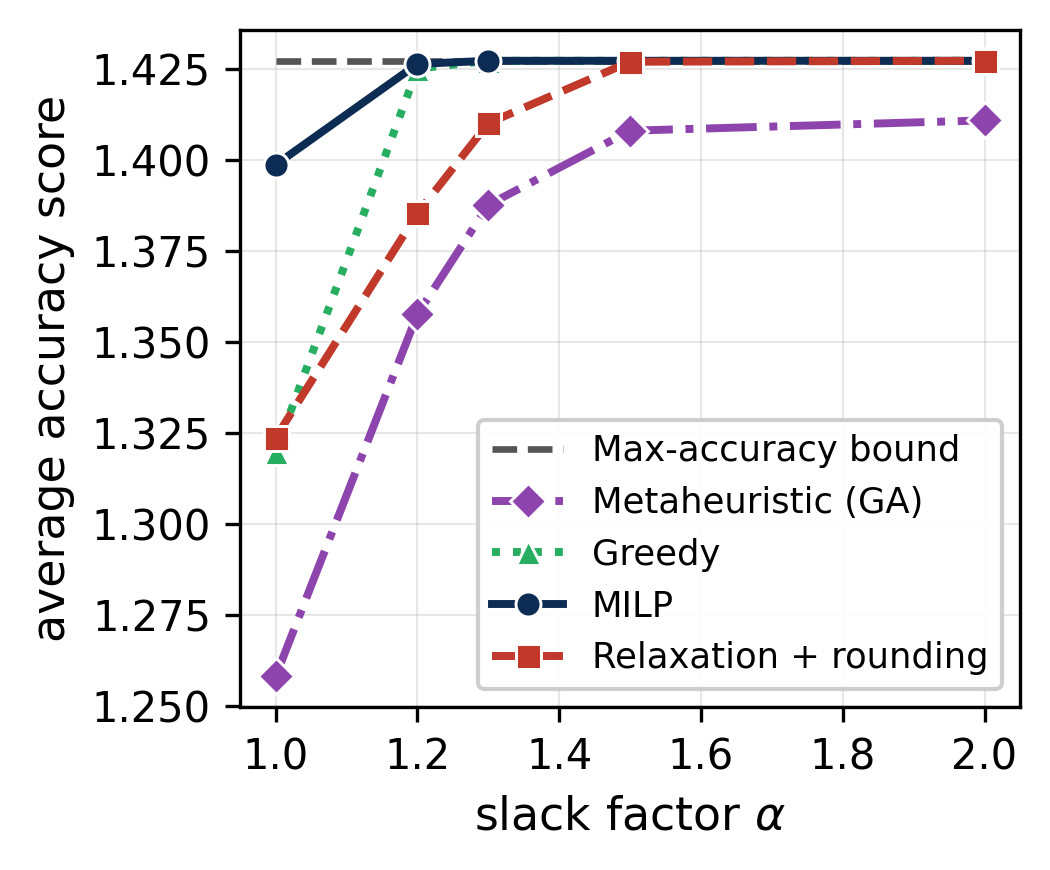
\includegraphics[width=\linewidth]{Figures/perf_slack_accuracy.png}}\hfill
\subcaptionbox{Accuracy vs.\ federation size $N$.\label{fig:nodes}}[0.28\textwidth]{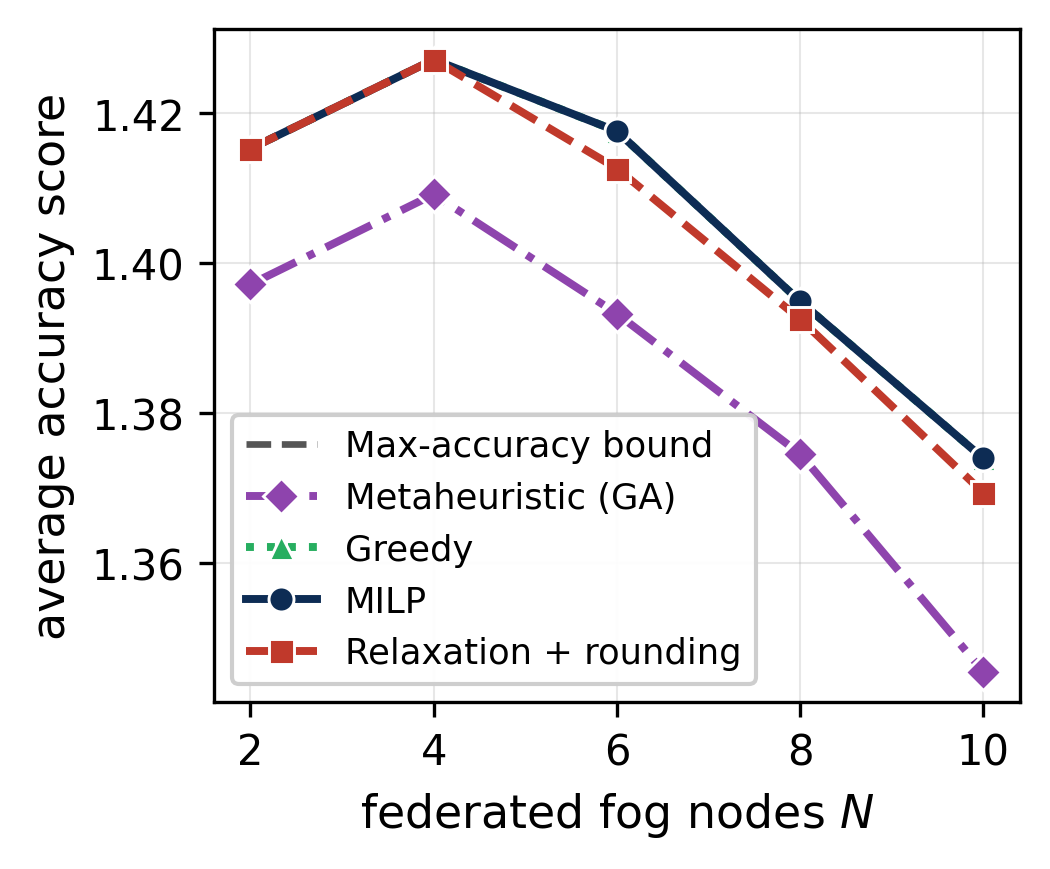
\includegraphics[width=\linewidth]{Figures/perf_nodes_accuracy.png}}\hfill
\subcaptionbox{Accuracy vs.\ workflow size $n$.\label{fig:tasksize}}[0.28\textwidth]{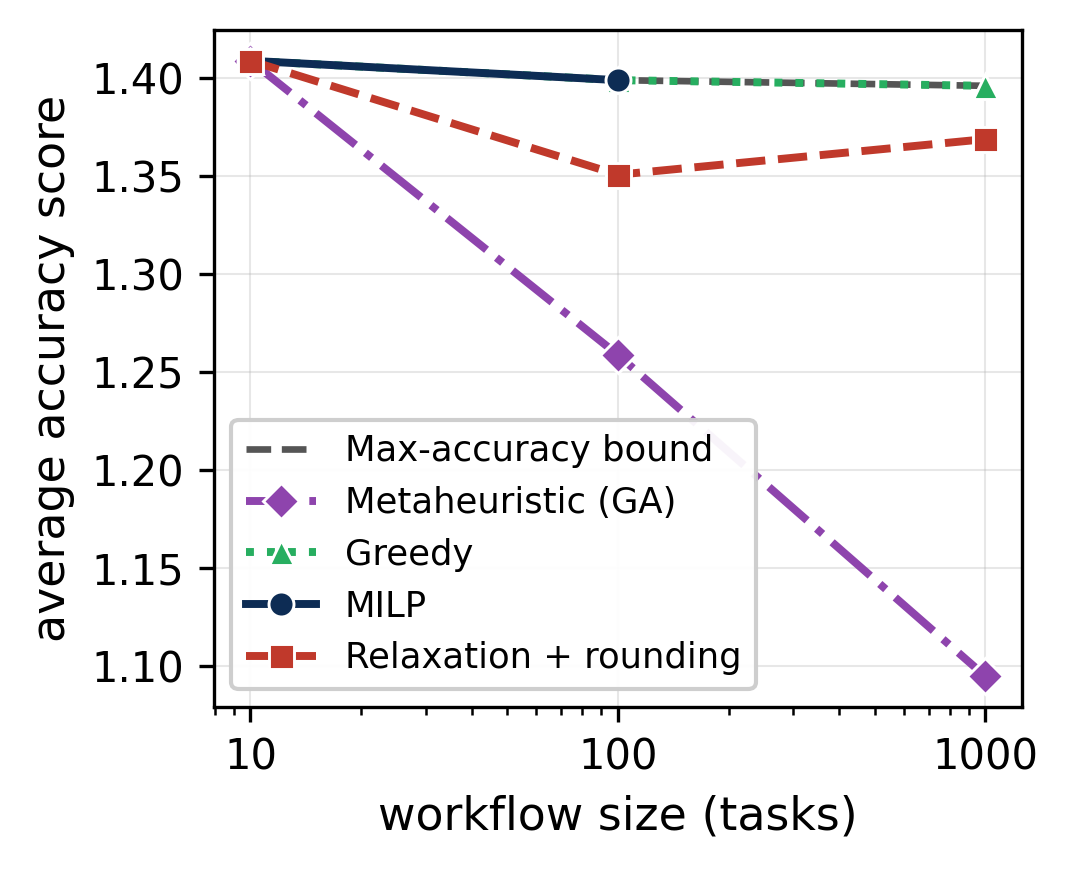
\includegraphics[width=\linewidth]{Figures/perf_task_size_acc_only.png}}\hfill
\subcaptionbox{Skipped tasks ($\ell_i{=}0$) per setting; they occur only in runs stopped at the time limit, never in certified optima.\label{fig:skipped}}[0.30\textwidth]{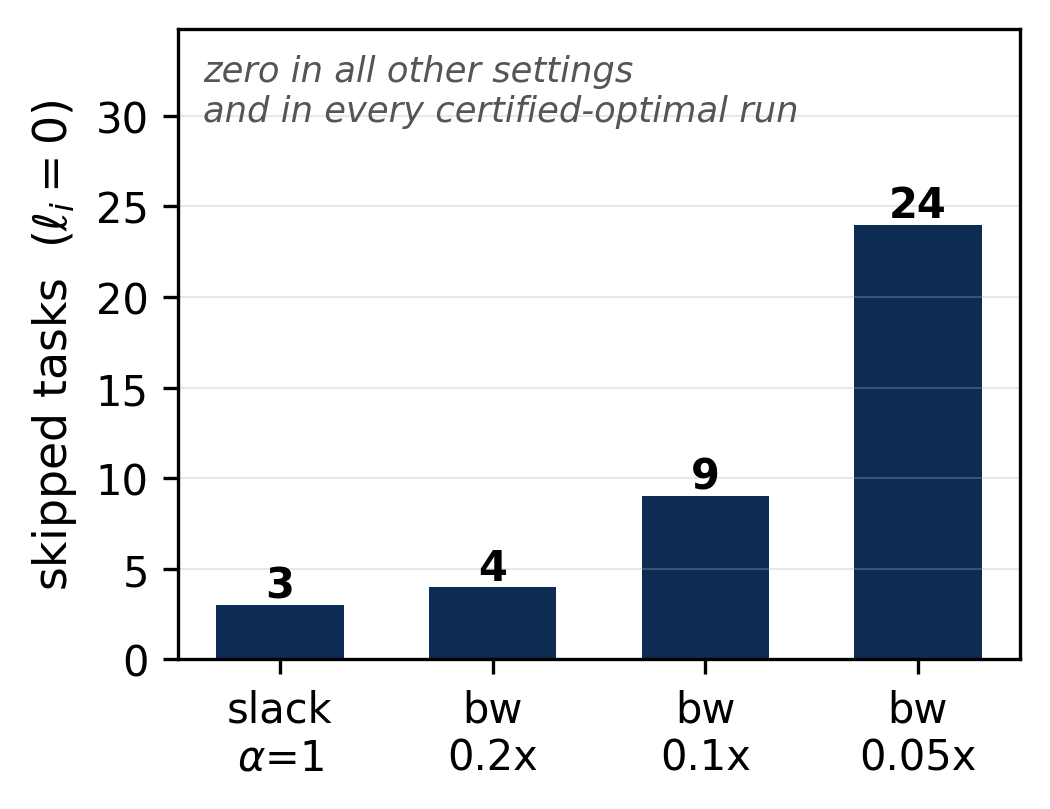
\includegraphics[width=\linewidth]{Figures/skipped_tasks.png}}\\[1ex]
\subcaptionbox{Accuracy (left) and deadline feasibility (right) vs.\ task failure rate.\label{fig:failure}}[0.44\textwidth]{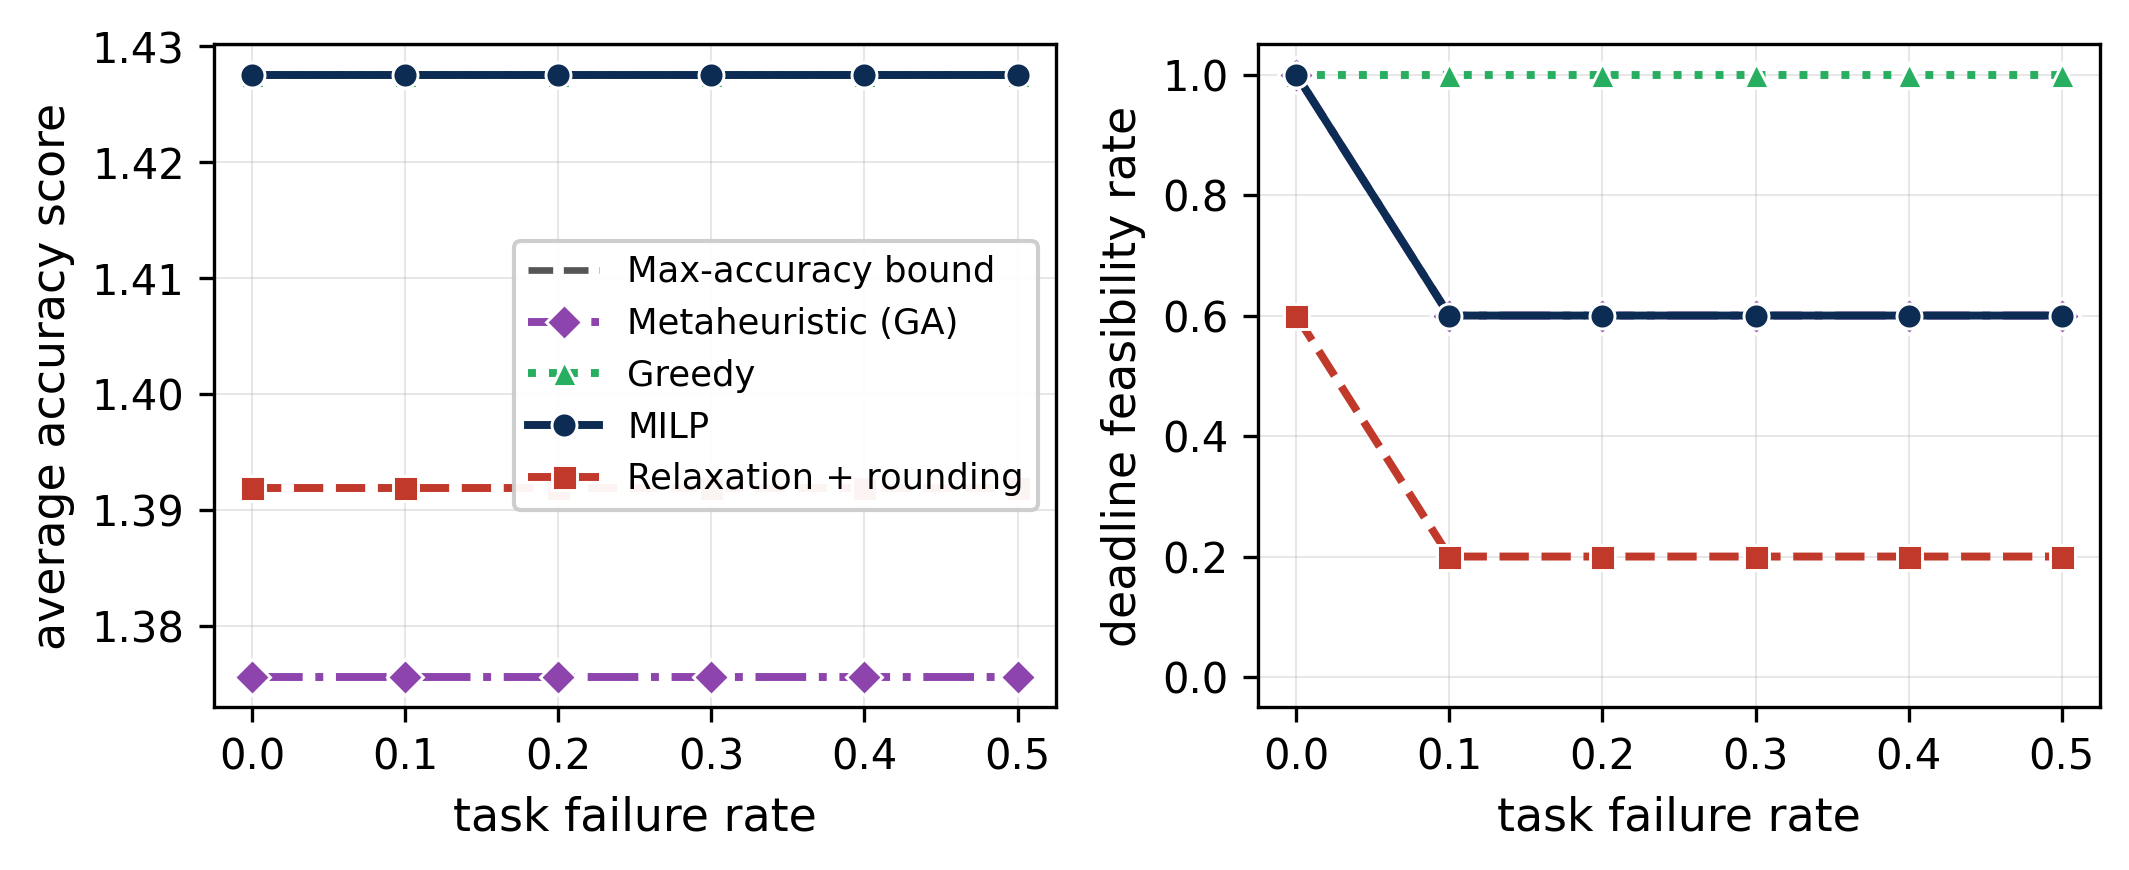
\includegraphics[width=\linewidth]{Figures/perf_failure_accuracy.png}}\hfill
\subcaptionbox{Accuracy (left) and deadline feasibility (right) as all link bandwidths are scaled down.\label{fig:bandwidth}}[0.44\textwidth]{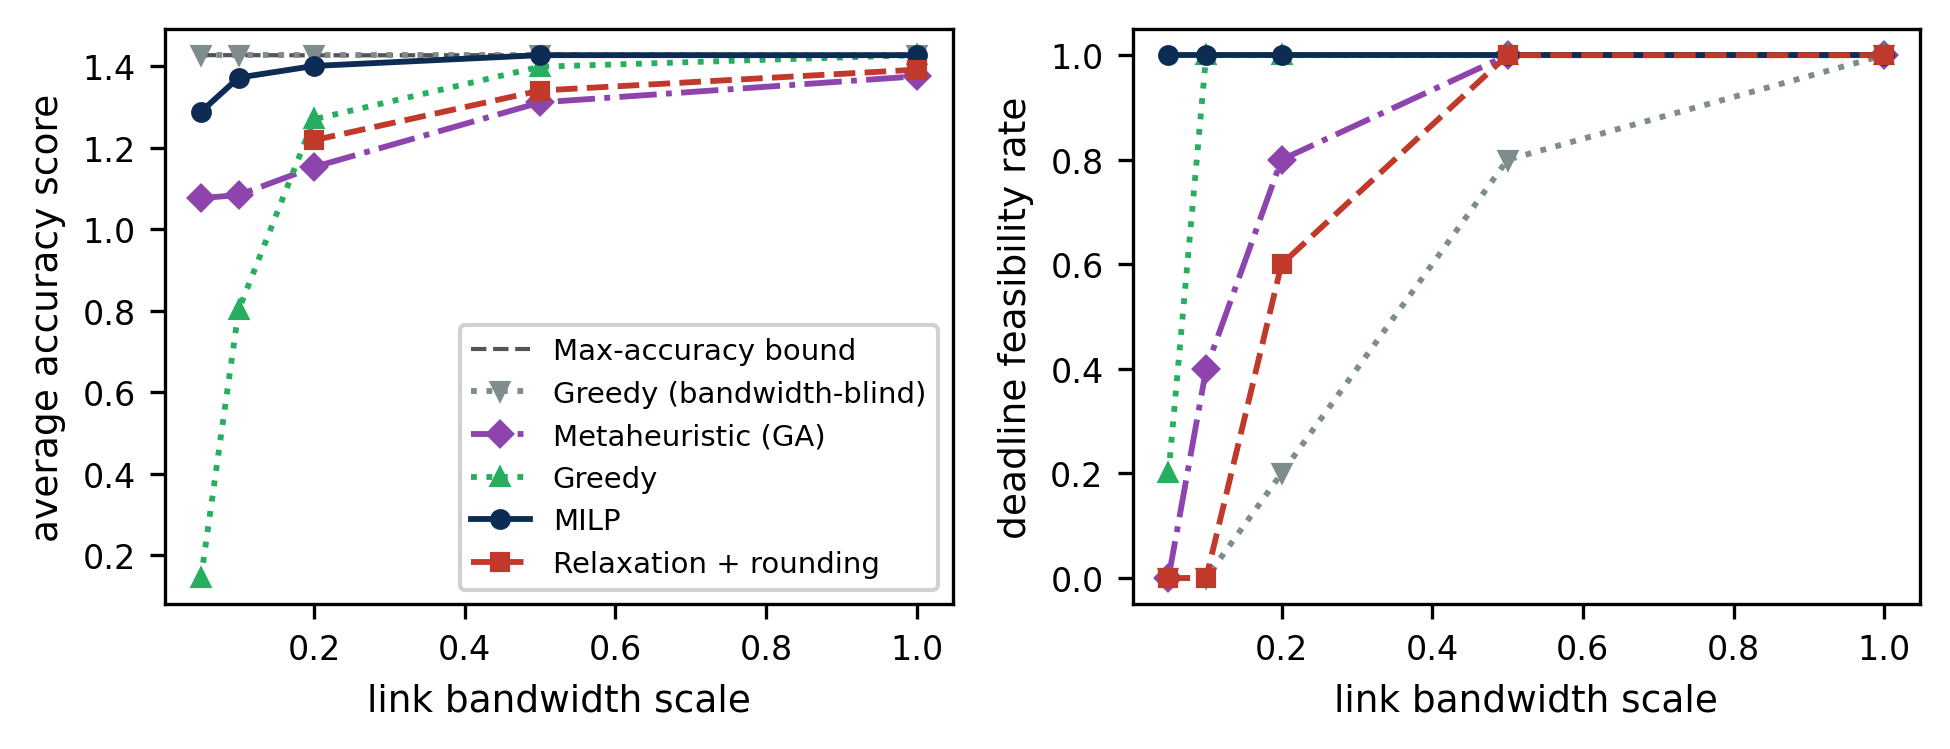
\includegraphics[width=\linewidth]{Figures/perf_bandwidth_accuracy.png}}
\caption{Reported average-accuracy score and deadline feasibility across the five experiments. The methods separate most when the deadline binds (a); extra nodes open placements rather than raising accuracy (b); the greedy tracks the bound at every size while answering in fractions of a second (c); under the retry-once model, retries preserve accuracy so methods separate on feasibility (d); and the bandwidth-blind baseline reports bound-level scores while missing the deadline below half bandwidth, where the data-aware methods trade accuracy for feasibility (e).}
\label{fig:experiments}
\end{figure*}

\subsection{Task Failures}

We model failures with a retry-once rule: when task $T_i$ fails on its node, it runs once more in place, paying $t_{ia}$ a second time, and it keeps its accuracy if the retry still finishes by the deadline. Fig.~\ref{fig:failure} shows score and deadline feasibility as the per-task failure rate rises from 0\% to 50\%. Scores do not move, since retries preserve accuracy; the methods separate on feasibility instead. The greedy is the only method whose schedule stays feasible at every rate: its placements leave enough slack to absorb the retries, while the MILP and the GA meet the deadline in about 60\% of runs once failures occur and rounding in about 20\%. The curves are nearly flat because at 50 tasks even a 10\% per-task rate makes at least one failure almost certain, so feasibility is decided by whether the schedule can absorb typical failure sets rather than by the rate itself.

\subsection{Link Bandwidth Degradation}
\label{sec:eval-bw}

The final experiment stresses the communication cost that motivates the model. On the default instance ($n{=}50$, $m{=}5$, $\alpha{=}1.5$), every inter-node bandwidth $B_{ba}$ is multiplied by a factor from 1.0 down to 0.05 while the deadline stays fixed, which is what a federation faces when links deteriorate during an event. To show what data-aware placement is worth, we add a bandwidth-blind baseline: the same greedy algorithm as Section~\ref{sec:greedy}, but choosing placements as if all transfers were free, and then evaluated against the real communication delays.

Fig.~\ref{fig:bandwidth} shows the two metrics that matter. On score alone, the blind baseline looks perfect---it runs every task fully and reports the bound at every level. The right panel shows why that is misleading: the blind schedules miss the deadline already at half bandwidth and are infeasible in every run at 0.1 and below. The data-aware schedulers behave differently. The MILP stays feasible at every level and loses only about 10\% of score at 0.05, shrinking execution fractions to fit the deadline. The greedy stays feasible down to 0.1 but pays in accuracy (0.80 at 0.1, mostly infeasible at 0.05). The GA is mostly feasible down to 0.1 and fails at 0.05. Rounding holds at 0.5, but its sampled assignments largely stop surviving the feasibility LP below that; this is a limit of our implementation, not a proof that no feasible rounding exists.

\subsection{Discussion}

The experiments point to three conclusions. First, the choice of
scheduler matters most when the deadline binds: at $\alpha{=}1.0$ the
methods separate with the MILP ahead, while by $\alpha{=}1.5$ the MILP
and the greedy coincide with the bound. Second, accuracy under a
binding deadline is not free in wall time: at 1000 tasks the greedy
finishes in about 0.15\,s, rounding spends about 372\,s per run, and
the GA about 159\,s for a markedly worse score. Third, under the
retry-once failure model the schedulers separate on feasibility rather
than accuracy, so placements that leave slack tolerate more failures.

\textbf{Bottlenecks and shortcomings.} The evaluation surfaced limits
that delimit where the formulation applies. (i)~\emph{MILP
scalability}: the model has $n\,N_{\mathrm{fog}}$ binary assignment
variables; we cap runs at 800 with a 60\,s limit (300\,s for
certification re-solves), and 18 of the 120 runs reached the limit, all
at $\alpha{=}1.0$ or under degraded bandwidth---exactly the hard
cases. (ii)~\emph{LP model size}: the relaxation introduces one
start-time constraint per (task, predecessor, node) triple, about
$10^5$ rows at $n{=}1000$; constraints must be assembled sparsely, a
cost rounding pays per trial. (iii)~\emph{Fixed GA budget}: the
population does not grow with $n$, which is why its score degrades in
Fig.~\ref{fig:tasksize}; size-adaptive budgets should close most of
that gap. (iv)~\emph{Failure semantics}: retry-once differentiates
schedulers through feasibility, but replication and checkpointing are
left out of the model. (v)~\emph{Dense instances}: per-edge data is
stored densely, so the $10^6$-task structures generated in the notebook
cannot yet be carried as schedulable instances; sparse storage and
decomposed formulations would extend the same model to genuinely large
deployments.

\section{Conclusion and Future Work}

This paper formulated data- and bandwidth-aware scheduling of approximate DAG workflows in federated fog systems as a mixed-integer linear program, and gave three scalable schedulers built on the same cost model. In simulation, the MILP earns a clear accuracy advantage when deadlines are tight; with generous slack the MILP and the greedy coincide at the bound; and at large workflow sizes the lightweight greedy holds its own while the GA's fixed search budget becomes its weakness. Under the retry-once failure model, the schedulers separate on deadline feasibility rather than accuracy.

Together, these results close the loop on the problem set out in the introduction: placements now pay the true cost of moving data between fog sites---the blind baseline shows what goes wrong without that term---and the execution fraction lets a workflow finish at reduced accuracy when full quality would miss the deadline.

Future work follows the shortcomings documented above: sparse storage and decomposed formulations to reach the $10^6$-task graphs we can already generate structurally; adaptive GA budgets that scale with $n$; richer failure semantics such as replication and checkpointing; and online re-scheduling with validation on a real federated fog testbed.

\section*{Acknowledgments}

This research is supported by the National Science Foundation (NSF).

\appendix
\section{Correctness and Linearization}
\label{app:proofs}
This appendix shows that the formulation of Section~\ref{sec:milp} means
what it should, and how to write it for a standard MILP solver. A
solution is \emph{feasible} if every task is placed on exactly one
permitted node, at most one $l_{ia}$ per task is non-zero, and all tasks
complete by $t_{\max}$.

\begin{lemma}
\label{lem:wellformed}
In any feasible solution: (i) $P_{ia}=0\Rightarrow e_{ia}=0$;
(ii) each task is assigned to exactly one node;
(iii) at most one $l_{ia}$ per task is non-zero, and
$l_{ia}>0\Rightarrow e_{ia}=1$;
(iv) the start time $M_{ia}$ respects data arrival, so $T_i$ cannot
start on $f_a$ before every predecessor has completed and its output
has reached $f_a$;
(v) on the node that runs $T_i$, $M_{ia}\le y_i$ and
$y_i=M_{ia}+t_{ia}l_{ia}$ is its completion time; and
(vi) every task completes by $y_i\le t_{\max}$.
\end{lemma}
\begin{proof}
(i) follows from \eqref{eq:elig}, (ii) from \eqref{eq:one}, and (iii)
from \eqref{eq:frac} with (ii). For (iv), induct on the distance from a
source: a source has $M_{ia}=0$ by \eqref{eq:startsrc}; for any other
task, \eqref{eq:start} gives
$M_{ia}\ge\max_{j\in\mathrm{in}_i}(y_j+\sum_{b}e_{jb}c_{ji}^{ba})$,
exactly the data-arrival bound. (v) is \eqref{eq:compl}, (vi) is
\eqref{eq:deadline}. The model only lower-bounds $M_{ia}$; the
earliest-start schedule is a special case.
\end{proof}

\begin{theorem}
\label{thm:correspondence}
Feasible solutions of \eqref{eq:obj}--\eqref{eq:bin} and valid schedules
are in one-to-one correspondence, and the optimal value of
\eqref{eq:obj} is the maximum achievable average weighted accuracy.
\end{theorem}
\begin{proof}
Lemma~\ref{lem:wellformed} shows a feasible $(e,l,M,y)$ is a valid
schedule whose accuracy \eqref{eq:obj} counts exactly. Conversely, from
any valid schedule set $e_{ia}=1$ on the node running $T_i$, $l_{ia}$
to the fraction executed, $M_{ia}$ and $y_i$ to the realized times;
validity implies \eqref{eq:one}--\eqref{eq:bin} with equal objective
value. The two sets correspond, so the MILP optimum equals the best
achievable accuracy.
\end{proof}

For an MILP solver, \eqref{eq:compl} contains the quadratic products
$e_{ia}M_{ia}$. With $U=t_{\max}+\max_{j,i,b,a}\{c_{ji}^{ba}\}$, bound
\begin{align}
M_{ia} &\le U, && \forall f_a,\ T_i, \label{eq:Mia}
\end{align}
introduce $z_{ia}=e_{ia}M_{ia}$, and replace \eqref{eq:compl} with
\begin{align}
y_i&=\sum_{f_a\in F} z_{ia}+\sum_{f_a\in F} t_{ia}l_{ia}, && \forall T_i, \label{eq:compllin}
\end{align}
together with the standard big-$M$ constraints
\begin{align}
0 \le z_{ia} &\le e_{ia} \, U, && \forall f_a,\ T_i, \label{eq:z1} \\
M_{ia}-(1-e_{ia})\,U \le z_{ia} &\le M_{ia}, && \forall f_a,\ T_i. \label{eq:z2}
\end{align}

\begin{theorem}
\label{thm:lin}
The linearized formulation admits exactly the same feasible $(e,l)$
pairs as \eqref{eq:obj}--\eqref{eq:bin}, and attains the same optimal
value of \eqref{eq:obj}.
\end{theorem}
\begin{proof}
No $M_{ia}$ needs to exceed $U$: every lower bound in \eqref{eq:start}
is at most $y_j+\max c_{ji}^{ba}\le U$, so larger values can be clamped
without touching the objective, and $M_{ia}\ge 0$ holds by
\eqref{eq:startsrc}--\eqref{eq:start}. When $e_{ia}=1$,
\eqref{eq:z2} squeezes $z_{ia}=M_{ia}=e_{ia}M_{ia}$; when $e_{ia}=0$,
\eqref{eq:z1} forces $z_{ia}=0=e_{ia}M_{ia}$. Hence
$z_{ia}=e_{ia}M_{ia}$ in all cases, and since $l_{ia}=0$ whenever
$e_{ia}=0$ by \eqref{eq:frac}, \eqref{eq:compllin} reduces to
\eqref{eq:compl}. Every other constraint is shared by both
formulations, so their feasible $(e,l)$ sets and optima coincide.
\end{proof}

\enlargethispage{8\baselineskip}
{\scriptsize
\linespread{0.85}\selectfont
\setlength{\itemsep}{0pt}
\bibliographystyle{ieeetr}
\balance
\bibliography{cas-refs}}

\end{document}